\documentclass[11pt]{article}
\usepackage{times, graphicx,float, multicol}
\usepackage[rflt]{floatflt}
\usepackage{hyperref}


\setlength{\textwidth}{6.5in}
\setlength{\textheight}{9.0in}
\setlength{\topmargin}{-.5in}
\setlength{\oddsidemargin}{-.0600in}
\setlength{\evensidemargin}{.0625in}

\newcommand{\secref}[1]{Section~\ref{#1}}

\newcommand{\doublespace}{\baselineskip0.34truein}
\newcommand{\singlespace}{\baselineskip0.16truein}
\newcommand{\midspace}{\baselineskip0.24truein}
\newcommand{\midplusspace}{\baselineskip0.26truein}

\def\TreeSearch{{TreeSearch}}

\title{{\TreeSearch} User Guide\\ {\large Version 1.0}}

\author{Derrick Stolee \\ 
	University of Nebraska-Lincoln\\ 
	\texttt{s-dstolee1@math.unl.edu}
       }
       
\begin{document}

\maketitle
\vspace{-.3in}
\begin{abstract}
	The {\TreeSearch} library abstracts the structure of a search tree
		in order to manage jobs in a distributed computation.
	This document details the strategy of {\TreeSearch} along with
		implementation, compilation, and execution details.
	An example application is also given.
\end{abstract}

\section{Introduction}
\label{sec:Introduction}

The computation path of a dynamic search frequently takes the form of a rooted tree.
One important property of each node in this tree is that the computation at that
	node depends only on the previous nodes in the ancestral path leading
	to the root of the computation.
If the search is implemented in the usual way, subtrees operate independently.

For a search of this type, all search nodes at a given depth 
	can be generated by iterating through the search tree, but 
	backtracking once the target depth is reached.
Each of the subtrees at this depth can be run independently,
	and hence it is common to run these jobs concurrently 
	(See \cite{ClassificationAlgorithms} Chapter 5 for more information).

The {\TreeSearch} library was built to maximize code reuse for these types of search.
It abstracts the structure of the tree and the recursive nature of the search into
	custom components available for implementation by the user.
Then, the ability to generate a list of jobs, run individual jobs, and submit the list
	of jobs to a cluster are available with minimal extra work.
	
{\TreeSearch} is intended for execution 
	on a distributed machine using
	Condor \cite{condor-practice},
	a job scheduler that uses idle nodes of a cluster or network.
Condor was chosen as its original development was meant for
	installation in computer labs and office machines 
	at the University of Wisconsin--Madison
	to utilize idle computers.
	
The C++ portion of {\TreeSearch} 
	is independent of Condor.
The Python scripts which manage the input and output files
	as well as modifying the submission script are
	tied to Condor, but 
	could be adapted for use in other schedulers.


\subsection{Acquiring \TreeSearch}

The latest version of {\TreeSearch} and its documentation
	is publicly available on GitHub \cite{github} at the address
	\href{http://www.github.com/derrickstolee/TreeSearch/}{http://www.github.com/derrickstolee/TreeSearch/}.


\section{Strategy}
\label{sec:Strategy}

Let us begin by describing the general structure and process of an abstract
	tree-based search.
There is a unique root node at depth zero.
Each node in the tree searches in a depth-first, recursive manner.
There are a number of children to select at each node.
One may select this child through iteration or selecting via a numerical order.
Before searching below the child, a pruning procedure may be called to attempt to 
	rule out the possibility of a solution below that child.
Another procedure may be used to find if this node is a solution.
Now, the search recurses at this node until its children are exhausted 
	and the search continues back to its parent.
%The tree search process, what order are things called?

\subsection{Subtrees as Jobs}

%Talk about the job descriptions.
This tree structure allows for search nodes to be described via the 
	list of children taken at each node.
Typically, the breadth of the search will be small and these descriptions take very little space.
This allows for a method of describing a search node independently of 
	what data is actually stored by the specific search application.
Moreover, the application may require visiting the ancestor search nodes in order
	to have consistent data.
With the assumption that each subtree is computationally independent of other subtrees at the same level,
	one can run each subtree in a different process in order to achieve parallelization.
These path descriptions make up the input for the specific processes in this scheme.

\begin{floatingfigure}{3in}\centering
	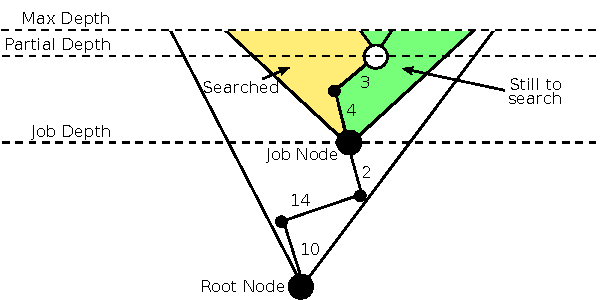
\includegraphics[width=3in]{figures/Jobs.pdf}
	\caption{\label{fig:jobs}A partial job description.}
\end{floatingfigure}


Each path to a search node qualifies as a single job, where the goal 
	is to expand the entire search tree below that node.
A collection of nodes where no pair are in an ancestor-descendant relationship 
	qualifies as a list of independent jobs.
Recognizing that the amount of computation required to expand 
	the subtree at a node is not always a uniform value,
	{\TreeSearch} allows a maximum amount of time 
	within a given job.
In order to recover the state of the search when the execution times out,
	the concept of \emph{partial jobs} was defined.
A partial job describes the path from the root to the current search node.
In addition, it describes which node in this path is the original job node.
The goal of a partial job is to expand the remaining nodes in the
	subtree of the job node, without expanding any nodes to 
	the left of the last  node in this path.
See Figure \ref{fig:jobs} to an example partial job and its position in the
	job subtree.

\subsection{Job Descriptions}

% How jobs/partials/solutions/completes/statistics are represented in the output

The descriptions of jobs and partial jobs are described using text files
	in order to minimize the I/O constraints on the distributed system.
The first is the standard job, given by a line starting with the letter \texttt{J}.
Following this letter are a sequence of numbers in hexadecimal.
The first two should be the same, corresponding to the depth of the node.
The remaining numbers correspond to the child values at each depth from the root to the job node.

A partial job is described by the letter \texttt{P}.
Here, the format is the same as a standard job except the first number describes the depth of the job node
	and the second number corresponds to 
	the depth of the current node.
For example, the job and partial job given in Figure \ref{fig:jobs} are described by the strings below:

\begin{verbatim}
    J 3 3 10 14 2
    P 3 5 10 14 2 4 3
\end{verbatim}

\subsection{Customization}

The {\TreeSearch} library consists of an iterative implementation of the abstract search.
The corresponding actions for a specific application are contacted via extending 
	the \texttt{SearchManager} class and implementing certain virtual functions.
The list of functions available are given in Table \ref{tbl:functions}.

	
\begin{table}[htb]\centering
\begin{tabular}[H]{|ll|p{3in}|}
	\hline
	\texttt{LONG\_T} & \texttt{pushNext()} & 
		Deepen the search to the next child of the current node.\\
	\hline
	\texttt{LONG\_T} & \texttt{pushTo(LONG\_T child)} & 
		Deepen the search to the specified child of the current node.\\
	\hline
	\texttt{LONG\_T} & \texttt{pop()} & 
		Remove the current node and move up the tree.\\
	\hline
	\texttt{int} & \texttt{prune()}  & 
		Perform a check to see if this node should be pruned.\\
	\hline
	\texttt{int} & \texttt{isSolution()} & 
		Perform a check to see if a solution exists at this point.\\
	\hline
	\texttt{char*} & \texttt{writeSolution()} & 
		Create a buffer that contains a description of the solution.\\
	\hline
	\texttt{char*} & \texttt{writeStatistics()}  & 
		Create a buffer that contains custom statistics.\\
	\hline
\end{tabular}
\caption{\label{tbl:functions}List of virtual functions in the \texttt{SearchManager} class.}
\end{table}


In addition to supplying the logic behind these functions, 
	protected members of the \texttt{SearchManager} class can be modified to change the
	operation of the search.
These parameters are listed in Table \ref{tbl:members}.

	
\begin{table}[htb]\centering
	\small
\begin{tabular}[H]{|lll|p{2.5in}|}
	\hline
	Type & Name & Option & Description\\
	\hline
	\texttt{int} & \texttt{maxdepth} & \texttt{-m [N]} &
		The maximum depth the search will go.  
		In generate mode, a job will be output with
		job description given by the current node. \\
	\hline
	\texttt{int} & \texttt{killtime} & \texttt{-k [N]} &
		Number of seconds before the search is halted.  
		If the search has not halted naturally, a partial job is output at the current node.\\
	\hline
	\texttt{int} & \texttt{maxSolutions} & \texttt{--maxsols [N]} &
		The maximum number of solutions to output.  
		When this number of solutions is reached, a partial job is output and the search halts.\\
	\hline
	\texttt{int} & \texttt{maxJobs} & \texttt{--maxjobs [N]} &
		The maximum number of jobs to output (generate mode).  
		When this number of jobs is reached, a partial job is output and the search halts.\\
	\hline
	\texttt{bool} & \texttt{haltAtSolutions} & \texttt{--haltatsols [yes/no]} &
	If \texttt{true}, the search will stop deepening if \texttt{isSolution()} signals a solution. 
	If \texttt{false}, the search will continue until specified by \texttt{prune()} or \texttt{maxdepth}.\\
	\hline
\end{tabular}
\caption{\label{tbl:members}List of members in the \texttt{SearchManager} class.}
\end{table}



\section{Integration with \TreeSearch}
\label{sec:Integration}

This section details the specific interfaces for
	implementation with {\TreeSearch}.

It is important to understand the order of events
	when the search is executing.
The search begins when the \texttt{doSearch()} methd
	is called.
The first call initializes the search, including
	starting the kill timer.
Then, each recursive call expands the current search node
	at the top of the stack.
Figure \ref{fig:doSearch} describes the actions
	taken by the recursive \texttt{doSearch()} 
	method takes at each search node.
	
\begin{figure}[p]
	\centering
	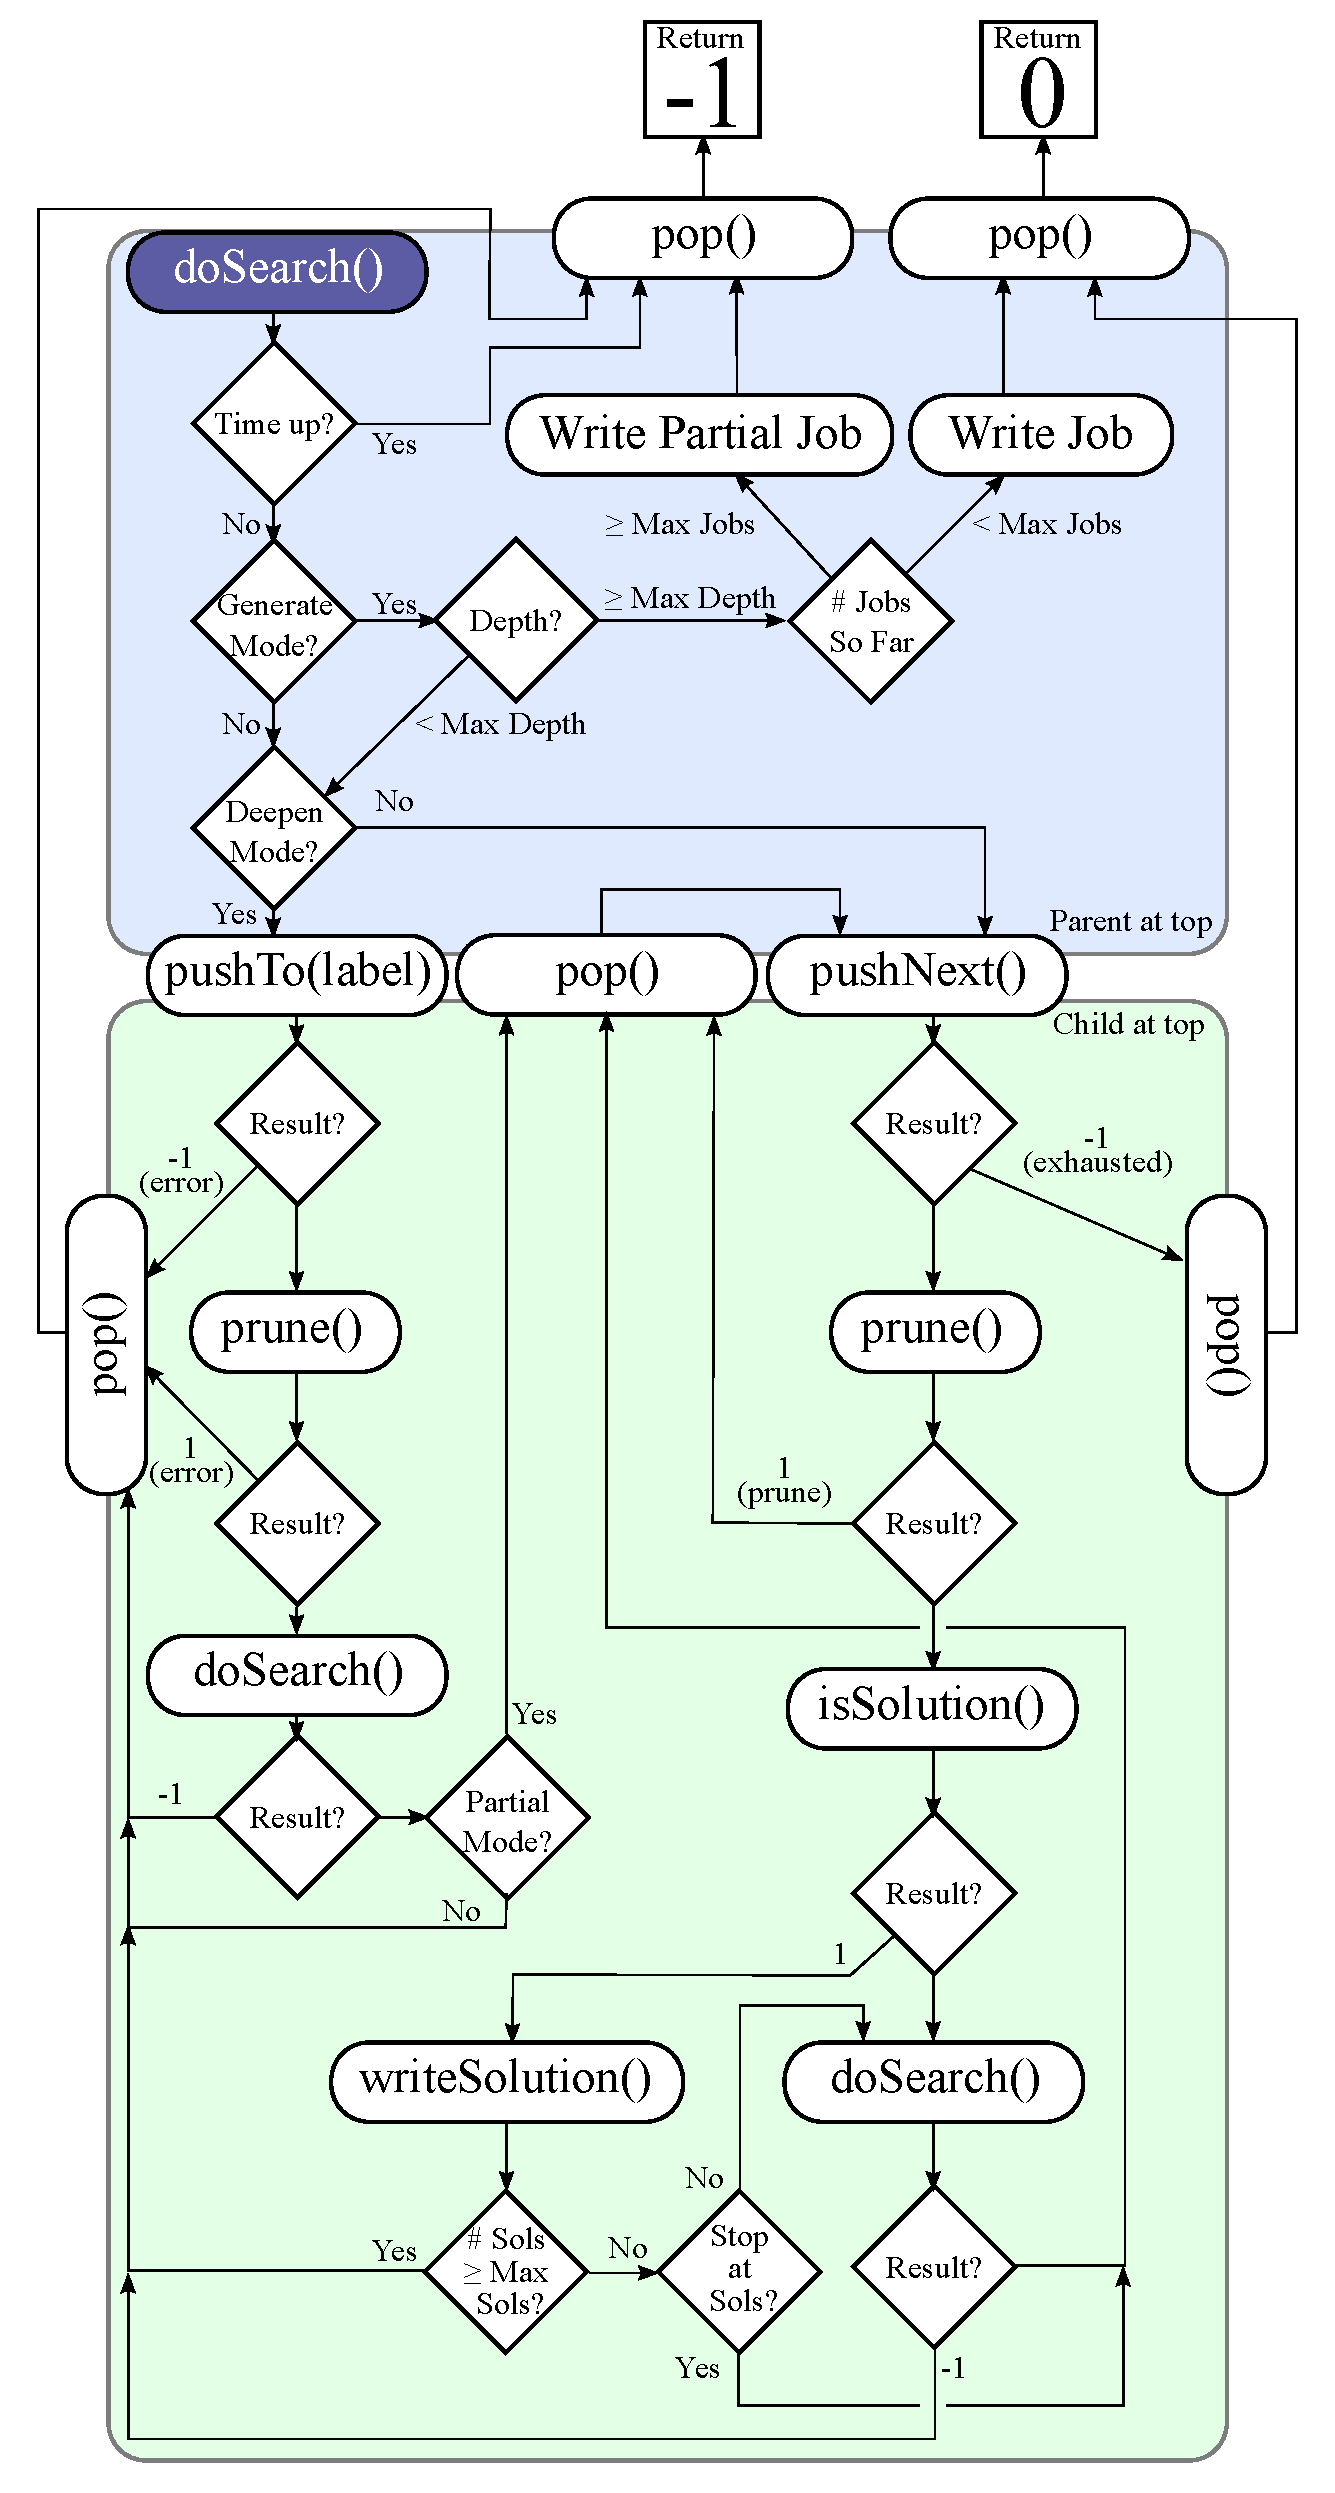
\includegraphics[height=0.95\textheight]{figures/doSearchFlowchart.pdf}
	\caption{\label{fig:doSearch}The operation of the \texttt{doSearch()} method.}
\end{figure}

\subsection{Virtual Functions}

The two most important methods are the
	\texttt{pushNext()} and \texttt{pushTo(LONG\_T child)} methods.
Both deepen the search, 
	manage the stack, 
	and control the job descriptions.
Each returns a child description (of type \texttt{LONG\_T})
	
	

	/**
	 * pushTo -- deepen the search to the specified child
	 * 	of the current node.
	 *
	 * @param child the specified label for the new node
	 * @return the label for the new node. -1 if none, or failed.
	 */
	virtual LONG\_T pushTo(LONG\_T child);

	/**
	 * pop -- remove the current node and move up the tree.
	 *
	 * @return the label of the node after the pop.
	 * 		This return value is used for validation purposes
	 * 		to check proper implementation of push*() and pop().
	 */
	virtual LONG\_T pop();

	/**
	 * prune -- Perform a check to see if this node should be pruned.
	 *
	 * @return 0 if no prune should occur, 1 if prune should occur.
	 */
	virtual int prune();

	/**
	 * isSolution -- Perform a check to see if a solution exists
	 * 		at this point.
	 *
	 * @return 0 if no solution is found, 1 if a solution is found.
	 */
	virtual int isSolution();

	/**
	 * writeSolution -- create a buffer that contains a
	 * 	description of the solution.
	 *
	 * Solution strings start with S.
	 *
	 * @return a string of data allocated with malloc().
	 * 	It will be deleted using free().
	 */
	virtual char* writeSolution();

	/**
	 * writeStatistics -- create a buffer that contains a
	 * 	description of the solution.
	 *
	 * Statistics take the following format in each line:
	 *
	 * T [TYPE] [ID] [VALUE]
	 *
	 * @return a string of data allocated with malloc().
	 * 	It will be deleted using free().
	 */
	virtual char* writeStatistics();




\subsection{Helper Methods}

The following methods are useful when constructing a {\TreeSearch} application.


/**
	 * importArguments -- take the command line arguments
	 * 	and convert them into options.
	 *
	 * This includes the following options:
	 * 	mode: generate or run
	 *  stages: -s [count] [s0] [s1] ... [sk]
	 *  killtime: -k [killtime]
	 *  maxdepth: -m [maxdepth]
	 *
	 *  It is set as virtual so that one can strip
	 *   custom arguments, if necessary.
	 */
	virtual void importArguments(int argc, char** argv);

	/**
	 * doSearch -- recursively perform the search from the current node.
	 *
	 * @return 1 if a solution is found, 0 if not.
	 */
	int doSearch();
	
	



\subsection{Compilation}
\label{sec:Compilation}

To compile \TreeSearch, run \texttt{make} in the source directory.
This command compiles the object file \texttt{treesearch.o} which must be
	linked into your executable.
Your code must reference the header file \texttt{treesearch.h}.
Moreover, it compiles the example application presented in Section \ref{sec:Example}.

\section{Execution and Job Management}
\label{sec:Execution}

To execute a single process, simply run your executable with the proper arguments.
However, to run a distributed job via Condor, a set of scripts were created to manage
	the input and output files, the Condor submission file, and monitor the progress
	of the submission during execution.

\subsection{Management Scripts}


The {\TreeSearch} library works best with independent subtrees
	 and hence does not suffer from scaling issues when the parallelism is increased.
However, managing these large lists of jobs requires automation.

\subsubsection{Expanding jobs before a run}

When the generation step is run, a list of jobs is presented in a single file.
Condor requires a separate input and output file for each process.
The role of the \texttt{expandjobs.py} script is to split the jobs into individual 
	files and to set up the Condor submission file for the number of jobs that are found.

There are a few customizable options for this script.

\begin{itemize}
	\item \texttt{-f [folder]} -- change the folder where the jobs are created.  Default is \texttt{./jobs}.
	\item \texttt{-m [maximum]} -- set the maximum number of jobs allowed.  Default is 500.
\end{itemize}

Inside the specified folder, the file \texttt{condorsubmit.sub} is set with
	the proper folder and queue size based on the number of jobs found.
Any remaining jobs that did not fit within the maximum are held as back jobs.
They will be added to the job pool when the jobs are completed.

\subsubsection{Collecting data after a run}

Once Condor has completed the requested jobs, the output must be collected to 
	discover which jobs completed fully, which are partially complete,
	and how many solutions have been found.
The script \texttt{compactjobs.py} was built for this purpose.

This script takes the output files and reads all new jobs that may have been generated 
	using the staging feature, finds if the input job completed or is partial,
	and reports on the total number of jobs of each type.
Moreover, it will find and store the solutions found, along with the corresponding data.

Finally, it compiles statistics from each run.  
Using the \texttt{writeStatistics} method,
	the application may report statistics by starting the line with a ``T" followed by the
	type (MAX, MIN, SUM), variable name, and variable value.
These are collected using the specified type and compiled with existing statistics from previous batches.






\section{Example Application}
\label{sec:Example}



\section{Example Workflow}
\label{sec:workflow}

Create submission template

---->

Generate initial jobs

---->

Compact data

---->

Evaluate \# of Jobs

---->

Expand with -M/-G

---->

RUN  --OR-- GENERATE (modify the condorsubmit.sub)

---->

BACK TO COMPACT

DURING A RUN:

check.sh

AFTER A RUN:

stats.sh/stataccept.txt


PREDICTING TIME:

randomjobs.py


\section{Summary}
\label{sec:Summary}


\section{Acknowledgements}

This software was developed with the support of the National Science Foundation grant DMS-0914815
	under the advisement of Stephen G. Hartke.

The author thanks the faculty and staff
	at the Holland Computing Center,
	especially David Swanson, Brian Bockleman, and Derek Weitzel for their extremely helpful advice
	during the design and development of this library.




\bibliographystyle{plain}
\bibliography{bibliography.bib}


\end{document}
